\section{Experiments and Results}

We conducted a variety of experiments to audit our previously
described approach. As a running example we used a DNN which we
trained on images from a generated dataset we dubbed \emph{Picasso
  Dataset}. The foundation are images of human faces we took from the
FASSEG dataset~\cite{khan2015multi,khan2017head}.
The Picasso Dataset contains collage images of faces with the facial
features (eyes, mouth, nose) either in the correct constellation
(positive class) or in a mixed-up constellation (negative class). See
Fig.~\ref{fig:picasso} for examples.
No distinction is made between originally left and right eyes.

\begin{figure}
  \begin{center}
    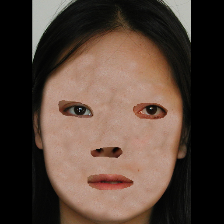
\includegraphics[width=.15\textwidth]{pic_00001_pos.png}\quad
    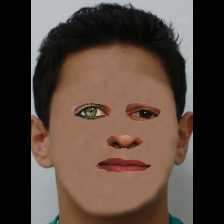
\includegraphics[width=.15\textwidth]{pic_00009_pos.png}\qquad\qquad
    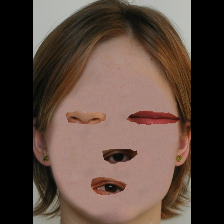
\includegraphics[width=.15\textwidth]{pic_00000_neg.png}\quad
    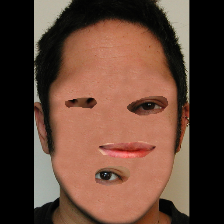
\includegraphics[width=.15\textwidth]{pic_00001_neg.png}
  \end{center}
  \caption{Examples from the Picasso Dataset
    (\textit{left:} positive class, \textit{right:} negative).}
  \label{fig:picasso}
\end{figure}

In order to not establish a divergence in the image space of the two
classes, the positive and negative classes contain facial features
that were cut out of a set of images from the original FASSEG
dataset. As a canvas to include the features, we took a set of
original faces and got rid of the facial features by giving the
complete facial area a similar skin-like texture. Then we included the
cut out facial features onto the original positions of the original
features in the faces.

The face images in Fig.~\ref{fig:picasso} show that
the resulting dataset is rather constructed. This however will suffice for
a proof of concept to show that our approach in fact exploits object parts
and their relations. In the future we plan on moving towards more natural
datasets.

\subsection{Analyzed DNNs}
We evaluated our method on three different architectures from the pytorch
model-zoo\footnote{\url{https://pytorch.org/docs/stable/torchvision/models.html}}:
AlexNet~\cite{krizhevsky_one_2014},
VGG16~\cite{simonyan_very_2015}, and
ResNeXt-50~\cite{xie_aggregated_2017}.
The convolutional parts of the networks were initialized with weights
pre-trained on the ImageNet dataset.
For fine-tuning the DNNs for the Picasso Dataset task,
% 
the output dimension was reduced to one and the in- and output
dimension of the second to last hidden dense layer was reduced to 512
for AlexNet and VGG16.
Then the dense layers and the last two convolutional layers
(AlexNet, VGG16) respectively bottleneck blocks (ResNeXt) were fine-tuned.
% 
The fine-tuning was conducted in one epoch on a training set of 18,002
generated, $224\times224$-sized picasso samples with equal
distribution of positive and negative class.
All models achieved accuracy greater than 99\%
on a test set of 999 positive and 999 negative samples.

% The fine-tuning failed for VGG16 when initialized with weights from
% the VGG face dataset, which we explain with the sub-optimal alignment
% of the objectives between VGG face and the Picasso Dataset.

\subsection{Training the Concept Models}
%%% Concept Data
In our example we determined the best ensembled detection concept vectors for
the concepts \textsc{eyes}, \textsc{mouth} and \textsc{nose} amongst the
considered layers.
% 
%%% Analyzed Model Layers
We excluded layers with low receptive field, as they are assumed to
hold only very local features
(for the layers used see Fig.~\ref{fig:layerwiseresults}).
Convolutional output was only considered after the activation.
% ResNeXt: starting at bottleneck modules 4/16,
% VGG16: starting at conv layer 5/13,
% AlexNet: starting at conv layer 2/5
% 
\begin{figure}%
  \centering%
  \hspace*{-0.08\textwidth}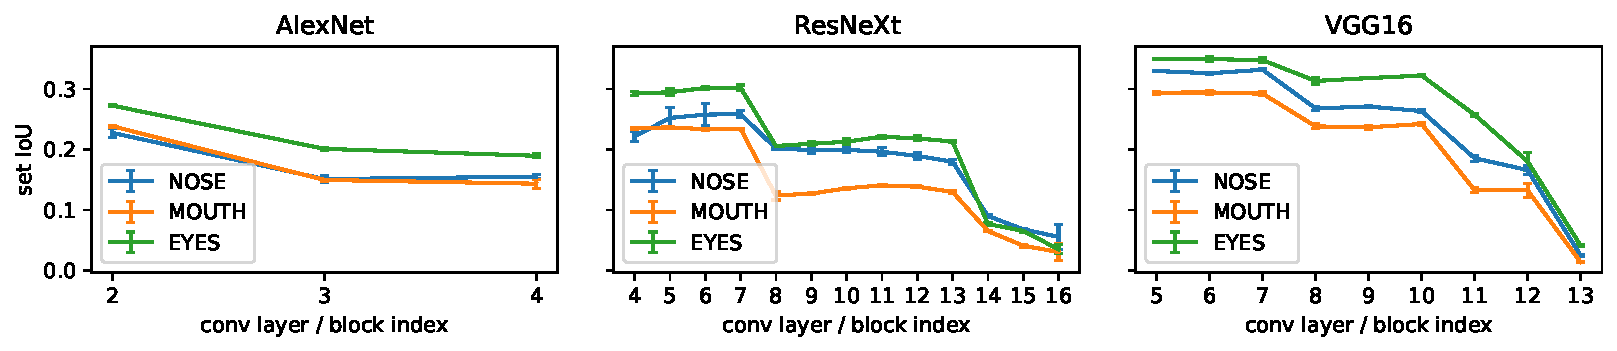
\includegraphics[width=1.16\textwidth]{layerwise_results_concept_embedding}
  \caption{The layer-wise mean set IoU results of the concept analysis runs.}
  \label{fig:layerwiseresults}
\end{figure}
% 
For each concept, 452 training/validation, and 48 test picasso samples
with segmentation masks were used.
% The concept window size determining the kernel size of the concept
% model convolution was chosen as the mean boxed size of the concept.
% The latter was chosen as
% $0.15\times0.05$ for the nose,
% $0.08\times0.2$ for the mouth, and
% $0.08\times0.16$ for an eye.
The training objective was: Predict at each activation map pixel
whether the kernel window centered there lies \enquote{over}
an instance of the concept. Over meant that the fuzzy intersection of
the concept segmentation and the kernel window area exceeds a threshold
(\emph{intersection encoding}).
This fuzzy definition of a box center
% introduces some noise to the ground truth, but
tackles the problem of sub-optimal intersections in later layers
due to low resolution.
% At a threshold greater or equal 0.5 masks are smoothed and sharpened.
Too high values may lead to elimination of an instance,
% Intersection over union (IoU) encoding is especially vulnerable to this for
% small concepts, wherefore we preferred intersection encoding.
and thresholds were chosen to avoid such issues with
values 0.5/0.8/0.7 for nose/mouth/eye.
We implemented the encoding via a convolution.
As evaluation metric we use set IoU (sIoU) between the detection
masks and the intersection encoded masks as in Net2Vec.
% 
%%% Optimization Method
On each dataset and each layer, 15 concept models were trained in
three 5-fold-cross-validation runs with the following settings:
Adam optimization with mean best learning rate of 0.001,
a weighting of 5:1 of Dice to bBCE loss,
batch size of 8, and
two epochs (all layers showed quick convergence).
% \begin{align*}
    %     \text{Loss}(M_\text{pred}, M)
    %     &= \lambda_\text{Dice} \text{Dice}(M_\text{pred}, M) +
            %             \lambda_\text{bBCE} \text{bBCE}(M_\text{pred}, M) \\
    %     \text{Dice}(M_\text{pred}, M)
    %           &= \frac{2\cdot MM_\text{pred}}
                  %                   {2\cdot MM_\text{pred} + (1-M)M_\text{pred} + M(1-M_\text{pred})} \\
    %     \text{bBCE}(M_\text{pred}, M)
    %           &= b M \log(M_\text{pred}) + (1-b) (1-M) \log(1-M_\text{pred})
                  %   \end{align*}
                  %                   for a ground truth intersection encoded mask $M$,
                  %                   a predicted mask $M_\text{pred}$,
                  %                   $b=0.99$ the mean proportion of background pixels in a concept mask
                  %                   (chosen for nose 0.999, else 0.995),
                  %                   and $\lambda_\text{Dice}=0.5$ and $\lambda_{bBCE}=0.1$.
                  %                   We recorded slightly worse results for higher weighting of the binary
                  %                   cross-entropy part or balancing of the Dice loss towards less false
                  %                   positives or less false negatives as described in
                  %                   \cite{salehi_tversky_2017}.
                  %                   

\paragraph{Results}
%%% ensemble performance pretty well coincides with mean performance, sometimes slightly better (possibly due to implicit confidence calibration)
Our normalized ensembling approach proved valuable as it yielded
mean or slightly better performance compared to the single runs.
For the considered models, meaningful embeddings of all concepts could
be found (see Tab.~\ref{tab:bestembeddings}): The layers all reached
sIoU values greater than 0.22
%%% influence of resolution
despite of the still seemingly high influence of sub-optimal
resolutions of the activation maps.
Fig.~\ref{fig:conceptsamples} shows some exemplary outputs.
%%% embeddings in early layers
The concepts were best embedded in earlier layers,
%%% embeddings in different layers
while different concepts did not necessarily share the same layer.
\begin{table}
  \centering
  \caption{Results for ensemble embeddings with
    set IoU (sIoU), mean cosine distance to the runs (Cos.d.),
    and index of conv layer or block (L) (cf. Fig.~\ref{fig:layerwiseresults}).
    \label{tab:bestembeddings}}%
  \footnotesize%
  \newcommand*{\normentry}[1]{\multicolumn{1}{c}{#1}}%
  \newcommand{\model}[1]{\multirow{4}{*}{
      \begin{tabular}{@{}c@{}}
        \rotatebox[origin=c]{90}{\strut#1}
      \end{tabular}}}%
  \newenvironment{statstable}[1]{%
    \begin{tabular}{@{}l >{\scshape}l c@{~~} S[table-auto-round] S[table-auto-round]@{}}%
      \toprule%
      \model{#1}
      & 
      & \normentry{L~~}
      & \normentry{sIoU}
      & \normentry{Cos.d.}\\%
      \cmidrule[\heavyrulewidth]{2-5}
    }{\bottomrule\end{tabular}}%
  \mbox{%
    \begin{statstable}{AlexNet}
      & nose  & 2 & 0.227925 & 0.04030534426371257 \\ % 0.290909
      & mouth & 2 & 0.239023 & 0.04018515348434448 \\ % 0.290484
      & eyes  & 2 & 0.271918 & 0.0581478198369344  \\ % 0.347822 
    \end{statstable}\hspace*{1em}%
    \begin{statstable}{VGG16}
      & nose  & 7 & 0.332171 & 0.10435034632682805 \\ % 0.468819
      & mouth & 6 & 0.295552 & 0.15369088053703306 \\ % 0.561507
      & eyes  & 6 & 0.349707 & 0.1969874024391174  \\ % 0.628199
    \end{statstable}\hspace*{1em}%
    \begin{statstable}{ResNeXt}
      & nose  & 6 & 0.263708 & 0.017367599999999928 \\ % 0.192076
      & mouth & 5 & 0.236788 & 0.020498533333333402 \\ % 0.208507
      & eyes  & 7 & 0.302339 & 0.019860466666666854 \\ % 0.205269
    \end{statstable}%
  }
\end{table}
\begin{figure}%
  \centering%
  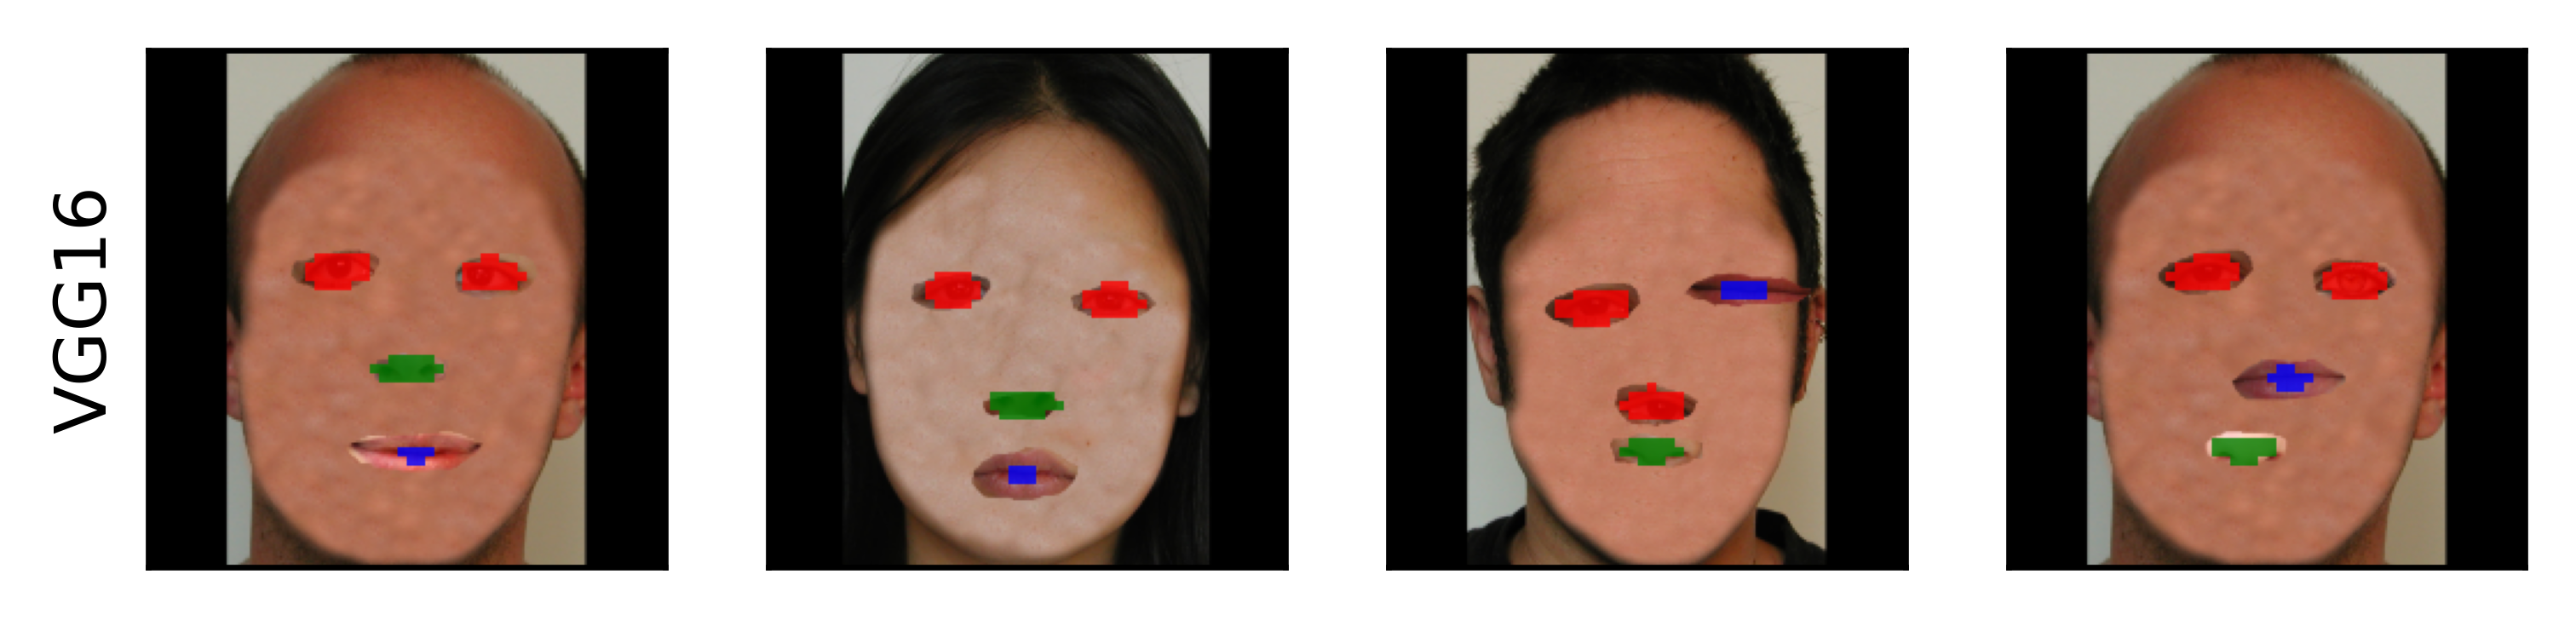
\includegraphics[width=0.6\textwidth]{vis_concept_predictions_vgg16}\\
  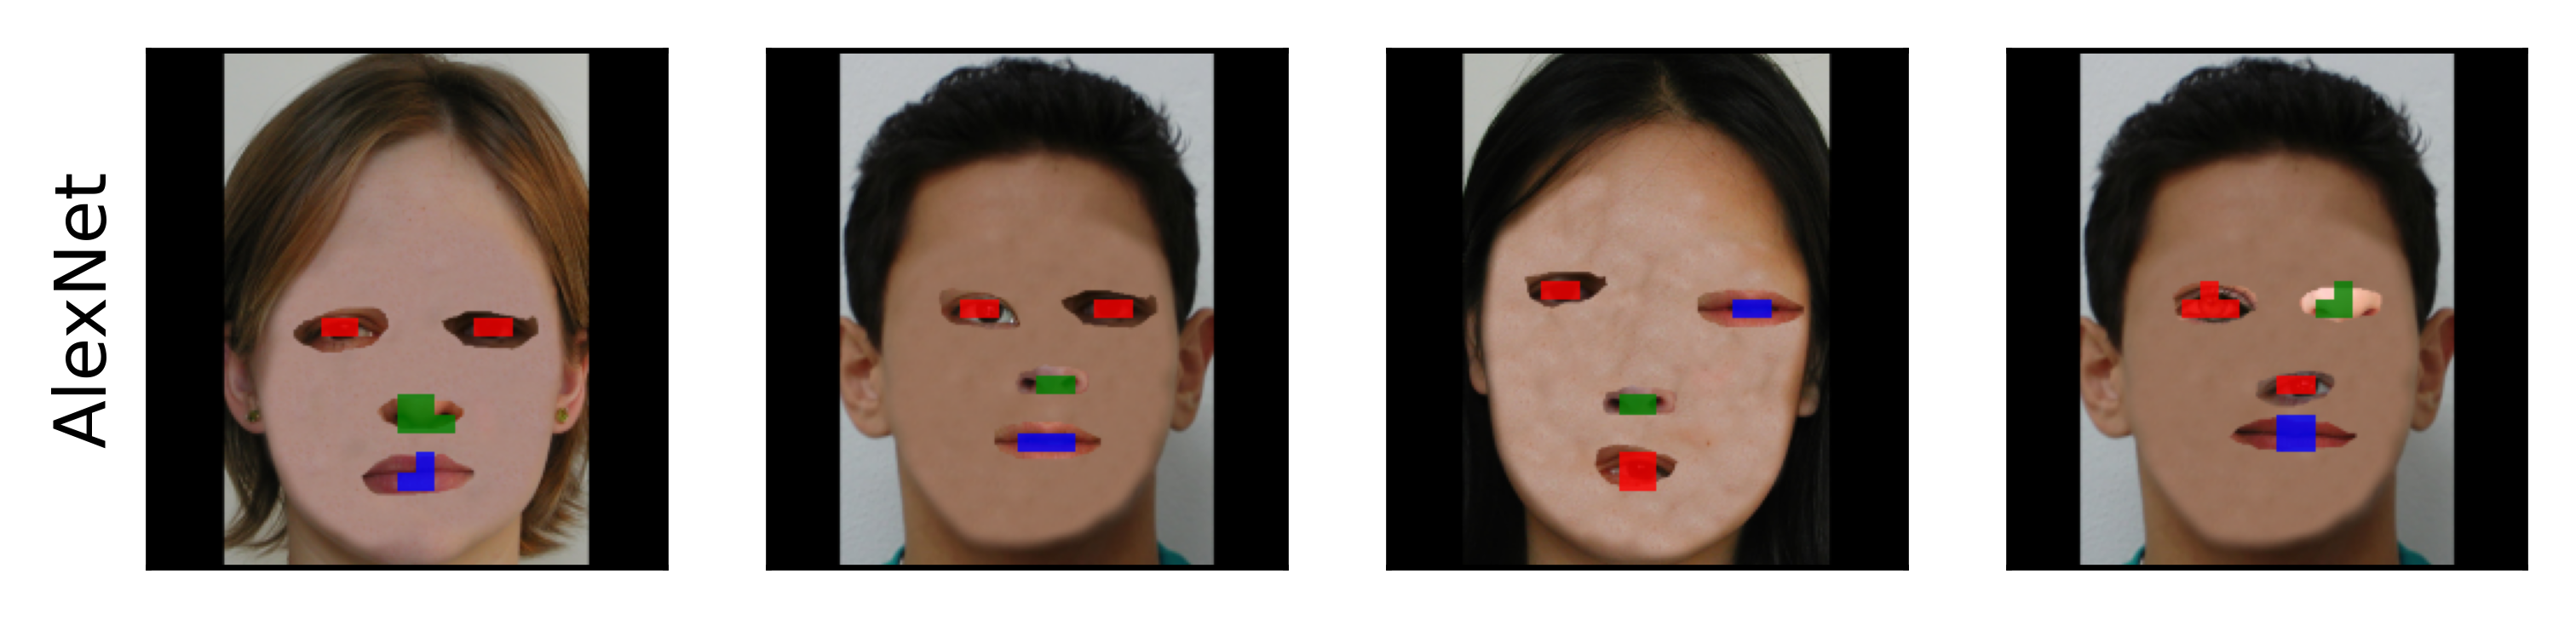
\includegraphics[width=0.6\textwidth]{vis_concept_predictions_alexnet}%
  \caption{
    Ensemble embedding outputs of
    \textsc{nose} (green), \textsc{mouth} (blue), \textsc{eyes} (red).}
  \label{fig:conceptsamples}
\end{figure}


\subsection{Example Selection for ILP Training}
The goal of the ILP model is to approximate the behavior of the main
DNN, \idest its decision boundary.
For this, few but meaningful training samples and their DNN output
are needed: class-prototypes as well as ones that tightly frame the
DNN decision boundary.
From the 1,998 samples in the picasso test set, in total 100 samples
were chosen from the DNN test set to train the ILP model.
The DNN confidence score here was used to estimate
the proximity of a data point to the decision boundary.
For each class, we selected the 50 samples predicted to be in this
class and with confidence closest to the class boundary of 0.5.
In our setup this provided a wide range of confidence values
(including 0 and 1).

\subsection{Finding the Symbolic Explanation}
In order to find the background knowledge needed for Aleph to generate
the explanation, we need to extract the information about the facial
features and their constellations from the masks of the samples drawn in the
previous step. Abiding the procedure described in
Sec.~\ref{sec:bkextraction}, we first find contiguous clusters in the
mask layers to then infer the positional information for them. This is
straight-forward for the nose and the mouth but imposes a problem for
the eyes, since we do not want to have a single position proposal for
them in the eye that produces the biggest cluster in the mask
layer. Thus, we allow for the top two biggest clusters to infer a
position. Although we give them unique constants in the BK, we both
give them the type \ilprule{eye} $\in C$.

The next step consists of the extraction of the spatial features
between the found parts. Since the relation pair
\ilprule{left\_of}\,/ \ilprule{right\_of} as well as
\ilprule{top\_of}\,/ \ilprule{bottom\_of} can be seen as the inverses of
the respective other relation, we omit the relations
\ilprule{right\_of} and \ilprule{bottom\_of} in the BK. This is
possible, because the \emph{Closed World Assumption} holds (Everything
that is not stated explicitly is false).

Once the BK is found for all examples, we can let Aleph induce a
theory of logic rules. Consider the induced theory for the trained
VGG16 network:
\ilprule{
  \begin{align*}
    \text{face(F) :- } &\text{contains(F, A), isa(A, nose), contains(F, B), isa(B, mouth),}\\
                       &\text{top\_of(A, B), contains(F, C), top\_of(C, A).}
  \end{align*}
}
The rule explicitly names the required facial concepts \ilprule{nose}
and \ilprule{mouth} and the fact that the nose has to be above the
mouth in order for an image to be a face. Further there is another
unnamed component \ilprule{C} required which has to be placed above
the nose. By construction this has to be one of the eyes. The rule
makes sense intuitively as it describes a subset of correct
constellations of the features of a human face.

To further test the fidelity of the generated explanations to the
original black-box network, we calculated several performance metrics
for a test set of 1998 test images (999 positive and 999 negative
examples). We handled the learned explanation rules as binary
classification model for the test images in BK representation. If an
image representation is covered by the explanation rules, it is
predicted to be positive, otherwise negative. We now can handle the
binary output of the black-box model as ground truth to our
explanation predictions. The performance metrics together with the
induced explanation rules for several DNN architectures are listed in
Tab.~\ref{tab:ilp_results}. It can be seen that the explanations stay
true to the original black-box model.

\begin{table}[t]
  \newcommand*{\rulepart}[1]{\ilprule{\scriptsize #1}}
  \caption{Learned rules for different architectures and their
    fidelity scores (accuracy and F1 score wrt.\ to the original model
    predictions).
    Learned rules are of common form
    \rulepart{face(F) :- contains(F, A), isa(A, nose), contains(F, B), isa(B, mouth), distinctPart}
  }
  \label{tab:ilp_results}
  \begin{tabular*}{\textwidth}{lcc@{\extracolsep{\fill}}l}
    \toprule
    \textbf{Arch.}   & \textbf{Accuracy} & \textbf{F1} & \textbf{Distinct rule part}\\
    \midrule[\heavyrulewidth]
    VGG16   & 99.60\%  & 99.60\%  & \rulepart{top\_of(A, B), contains(F, C), top\_of(C, A)} \\
    AlexNet & 99.05\%  & 99.04\%  & \rulepart{contains(F, C), left\_of(C, A), top\_of(C, B), top\_of(C, A)} \\
    ResNext & 99.75\%  & 99.75\%  & \rulepart{top\_of(A, B), contains(F, C), top\_of(C, A)}\\
    \bottomrule
  \end{tabular*}
\end{table}

% When it comes to explaining the network behavior it is
% particularly important to look at edge cases. This can be cases
% where the network is not sure about a prediction or is even
% wrong. We expect an explanation to accurately resemble the
% decisions of the original network. We therefore investigated if
% the false positives in the test set are correctly labeled as
% positives and the false negatives are correctly labeled as
% negatives by the explanation rules. This was in fact the case all
% occurring




%%% Local Variables:
%%% mode: latex
%%% TeX-master: "concept_embeddings_and_ilp"
%%% End:
